\section{Запись разрешающей системы уравнений МКЭ, проведение ее анализа и получение <<вручную>> решения для перемещений и напряжений}

Разрешающую систему МКЭ получим методом равновесия узлов. Для этого составим дискретную модель. За конечный элемент возьмем каждый участок длиной $l$:
\begin{figure}[H]
    \begin{center}
        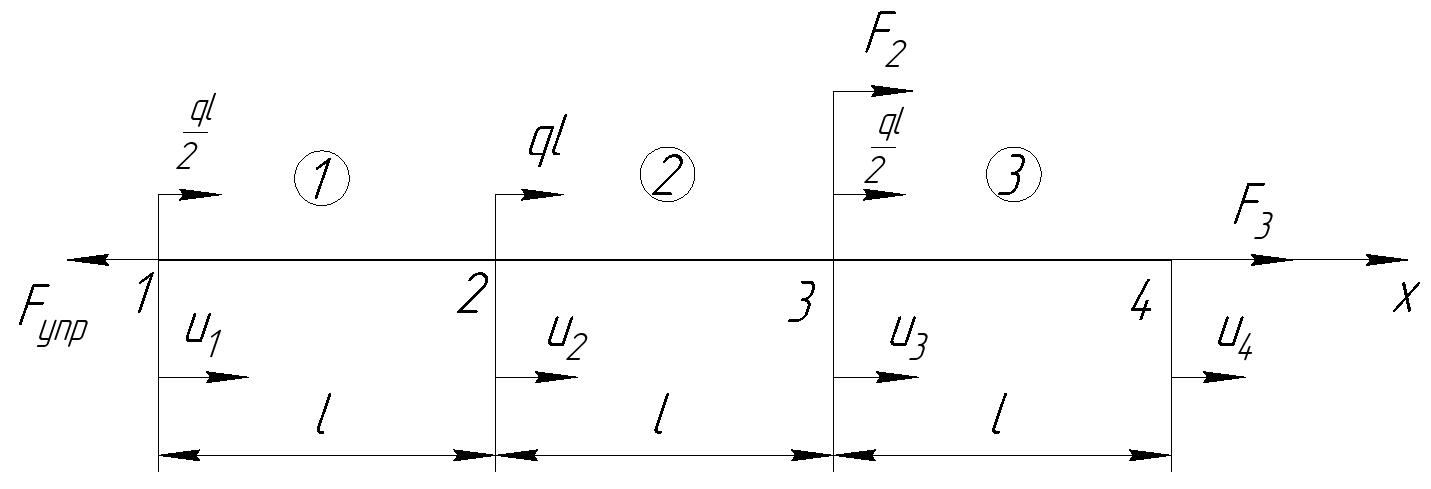
\includegraphics[width = 0.7\linewidth]{pic6.1.PNG}
        \caption{Дискретная модель}
        \label{pic6.1}
    \end{center}
\end{figure}

Разрежем модель на конечные элемнты и узлы:
\begin{figure}[H]
    \begin{center}
        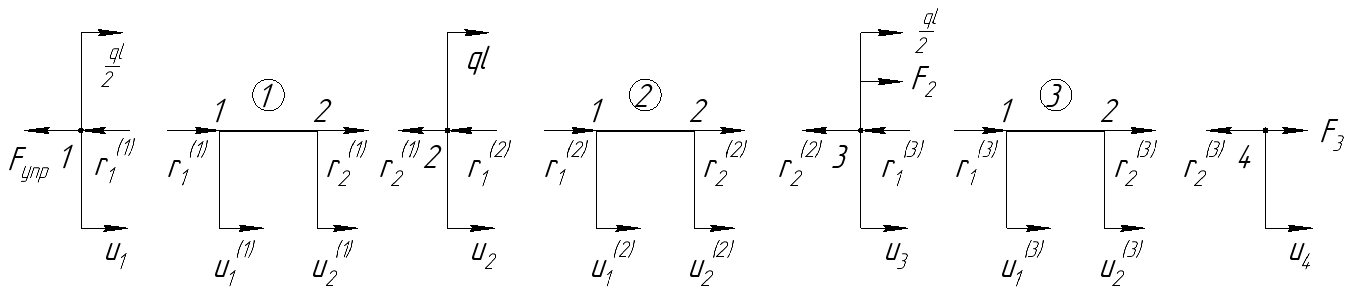
\includegraphics[width = \linewidth]{pic6.2.PNG}
        \caption{Разбиение дискретной модели на узлы и КЭ}
        \label{pic6.2}
    \end{center}
\end{figure}

Запишем условие равновесия для i-го КЭ:
\begin{equation}
    \label{eq6.1}
    \frac{EF}{l}
    \begin{bmatrix}
        1 & -1
        \\
        -1 & 1
    \end{bmatrix}
    \begin{Bmatrix}
        u_{1}^{(i)}
        \\
        u_{2}^{(i)}
    \end{Bmatrix}
    = 
    \begin{Bmatrix}
        r_{1}^{(i)}
        \\
        r_{2}^{(i)}
    \end{Bmatrix}
\end{equation}
или в обычном виде:
\begin{equation}
    \label{eq6.2}
    \begin{cases}
        \displaystyle \frac{EF}{l} (u_1^{(i)} - u_2^{(i)}) = r_1^{(i)}
        \\[10pt]
        \displaystyle \frac{EF}{l} (u_2^{(i)} - u_1^{(i)}) = r_2^{(i)}
    \end{cases}
\end{equation}

Запишем условия равновесия узлов:
\begin{equation}
    \label{eq6.3}
    \begin{cases}
        \displaystyle F_{\t{упр}} + r_1^{(1)} - \frac{ql}{2} = 0
        \\
        \displaystyle r_2^{(1)} + r_1^{(2)} - ql = 0
        \\
        \displaystyle r_2^{(2)} + r_1^{(3)} - F_2 - \frac{ql}{2} = 0
        \\
        \displaystyle r_2^{(3)} - F_3 = 0
    \end{cases}
\end{equation}

Подставим (\ref{eq6.2}) в (\ref{eq6.3}) и учтем, что $F_{\t{упр}} = c \cdot u_1$:
\begin{equation}
    \label{eq6.4}
    \begin{cases}
        \displaystyle cu_1 + \frac{EF}{l} (u_1^{(1)} - u_2^{(1)}) - \frac{ql}{2} = 0
        \\[10pt]
        \displaystyle \frac{EF}{l} (u_2^{(1)} - u_1^{(1)}) + \frac{EF}{l} (u_1^{(2)} - u_2^{(2)}) - ql = 0
        \\[10pt]
        \displaystyle \frac{EF}{l} (u_2^{(2)} - u_1^{(2)}) + \frac{EF}{l} (u_1^{(3)} - u_2^{(3)}) - F_2 - \frac{ql}{2} = 0
        \\[10pt]
        \displaystyle \frac{EF}{l} (u_2^{(3)} - u_1^{(3)}) - F_3 = 0
    \end{cases}
\end{equation}

Объединим все элементы в единую систему. Тогда будут выполняться следующие соотношения:
\begin{equation}
    \label{eq6.5}
    \begin{cases}
        u_1^{(1)} = u_1
        \\
        u_2^{(1)} = u_1^{(2)} = u_2
        \\
        u_2^{(2)} = u_1^{(3)} = u_3
        \\
        u_2^{(3)} = u_4
    \end{cases}
\end{equation}

Подставим (\ref{eq6.5}) в (\ref{eq6.4}):
\begin{equation}
    \label{eq6.6}
    \begin{cases}
        \displaystyle cu_1 + \frac{EF}{l} (u_1 - u_2) - \frac{ql}{2} = 0
        \\[10pt]
        \displaystyle \frac{EF}{l} (u_2 - u_1) + \frac{EF}{l} (u_2 - u_3) - ql = 0
        \\[10pt]
        \displaystyle \frac{EF}{l} (u_3 - u_2) + \frac{EF}{l} (u_3 - u_4) - F_2 - \frac{ql}{2} = 0
        \\[10pt]
        \displaystyle \frac{EF}{l} (u_4 - u_3) - F_3 = 0
    \end{cases}
\end{equation}

Сгруппируем коэффициенты при одинаковых перемещениях и перенесем нагрузку в правую часть:
\begin{equation}
    \label{eq6.7}
    \begin{cases}
        \displaystyle (c + \frac{EF}{l}) u_1 - \frac{EF}{l} u_2 = \frac{ql}{2}
        \\[10pt]
        \displaystyle - \frac{EF}{l} u_1 + 2 \frac{EF}{l} u_2 - \frac{EF}{l} u_3 = ql
        \\[10pt]
        \displaystyle - \frac{EF}{l} u_2 + 2 \frac{EF}{l} u_3 - \frac{EF}{l} u_4 = F_2 + \frac{ql}{2}
        \\[10pt]
        \displaystyle - \frac{EF}{l} u_3 + \frac{EF}{l} u_4 = F_3
    \end{cases}
\end{equation}

Запишем (\ref{eq6.7}) в матричном виде:
\begin{equation}
    \label{eq6.8}
    \begin{bmatrix}
        c + \matrfrac{EF}{l} & - \matrfrac{EF}{l} & 0 & 0
        \\[10pt]
        - \matrfrac{EF}{l} & 2 \matrfrac{EF}{l} & - \matrfrac{EF}{l} & 0
        \\[10pt]
        0 & - \matrfrac{EF}{l} & 2 \matrfrac{EF}{l} & - \matrfrac{EF}{l}
        \\[10pt]
        0 & 0 & - \matrfrac{EF}{l} & \matrfrac{EF}{l}
    \end{bmatrix}
    \cdot
    \begin{Bmatrix}
        u_1
        \\[10pt]
        u_2
        \\[10pt]
        u_3
        \\[10pt]
        u_4
    \end{Bmatrix}
    =
    \begin{Bmatrix}
        \matrfrac{ql}{2}
        \\[10pt]
        ql
        \\[10pt]
        F_2 + \matrfrac{ql}{2}
        \\[10pt]
        F_3
    \end{Bmatrix}
\end{equation}
Разделим (\ref{eq6.8}) на $\displaystyle \frac{EF}{l}$ учитывая (\ref{eq0.1}):
\begin{equation}
    \label{eq6.9}
    \begin{bmatrix}
        8 & -1 & 0 & 0
        \\
        -1 & 2 & -1  & 0
        \\
        0 & -1 & 2 & -1
        \\
        0 & 0 & -1 & 1
    \end{bmatrix}
    \cdot
    \begin{Bmatrix}
        u_1
        \\
        u_2
        \\
        u_3
        \\
        u_4
    \end{Bmatrix}
    =
    \begin{Bmatrix}
        \displaystyle \frac{l}{2}
        \\
        l
        \\
        l
        \\
        0.2l
    \end{Bmatrix}
\end{equation}

Искать решения для системы (\ref{eq6.9}) будем методом Крамера:
\begin{equation}
    \label{eq6.10}
    u_i = \frac{\Delta_i}{\Delta}
\end{equation}
\begin{equation}
    \label{eq6.11}
    \begin{split}
        & \Delta =
        \begin{vmatrix}
            8 & -1 & 0 & 0
            \\
            -1 & 2 & -1 & 0
            \\
            0 & -1 & 2 & -1
            \\
            0 & 0 & -1 & 1
        \end{vmatrix}
        = 8 \cdot
        \begin{vmatrix}
            2 & -1 & 0
            \\
            -1 & 2 & -1
            \\
            0 & -1 & 1
        \end{vmatrix}
        + 1 \cdot
        \begin{vmatrix}
            -1 & -1 & 0
            \\
            0 & 2 & -1
            \\
            0 & -1 & 1
        \end{vmatrix}
        =
        \\
        & = 8 \cdot [2 \cdot (2-1) + 1(-1)] + (-1)(2-1) + 1 \cdot 0 = 8 - 1 = 7
    \end{split}
\end{equation}
\begin{equation}
    \label{eq6.12}
    \begin{split}
        & \Delta_1 = 
        \begin{vmatrix}
            \displaystyle \frac{l}{2} & -1 & 0 & 0
            \\
            l & 2 & -1 & 0
            \\
            l & -1 & 2 & -1
            \\
            0.2l & 0 & -1 & 1
        \end{vmatrix}
        = \frac{l}{2} [ 2 \cdot (2 - 1) + 1 \cdot (-1) ] + 1 \cdot [l \cdot (2 - 1) + 1 \cdot (l + 0.2l)] = 
        \\
        & = 0.5l + 2.2l = 2.7l
    \end{split}
\end{equation}
\begin{equation}
    \label{eq6.13}
    \begin{split}
        & \Delta_2 = 
        \begin{vmatrix}
            8 & \displaystyle \frac{l}{2} & 0 & 0
            \\
            -1 & l & -1 & 0
            \\
            0 & l & 2 & -1
            \\
            0 & 0.2l & -1 & 1
        \end{vmatrix}
        = 8 \cdot [l \cdot (2 - 1) + 1 \cdot (l + 0.2l)] - 0.5l \cdot [-1 \cdot (2 - 1) + 1 \cdot (0)] =
        \\
        & = 8 \cdot (l + 1.2l) - 0.5l \cdot (-1) = 18.1l
    \end{split}
\end{equation}
\begin{equation}
    \label{eq6.13.1}
    \begin{split}
        & \Delta_3 =
        \begin{vmatrix}
            8 & -1 & \displaystyle \frac{l}{2} & 0
            \\
            -1 & 2 & l & 0
            \\
            0 & -1 & l & -1
            \\
            0 & 0 & 0.2l & 1
        \end{vmatrix}
        = -0.2l \cdot [1 \cdot 0 - 1 \cdot (8 \cdot 2 - 1)] + 1 \cdot [1 \cdot (8l + 0.5l) + l \cdot (8 \cdot 2 - 1)] = 
        \\
        & = -0.2l \cdot (-15) + 8.5l + 15l = 26.5l
    \end{split}
\end{equation}
\begin{equation}
    \label{eq6.13.2}
    \begin{split}
        & \Delta_4 =
        \begin{vmatrix}
            8 & -1 & 0 & \displaystyle \frac{l}{2}
            \\
            -1 & 2 & -1 & l
            \\
            0 & -1 & 2 & l
            \\
            0 & 0 & -1 & 0.2l
        \end{vmatrix}
        = 1 \cdot [1 \cdot (8l + 0.5l) + l \cdot (8 \cdot 2 - 1)] + 0.2l \cdot [1 \cdot (-8) + 2 \cdot (8 \cdot 2 - 1)] =
        \\
        & = 8.5l + 15l + 0.2l \cdot 22 = 27.9l
    \end{split}
\end{equation}
\begin{equation}
    \label{eq6.14}
    \begin{cases}
        \displaystyle u_1 = \frac{\Delta_1}{\Delta} = 0.386l = 0.193 \; \t{м}
        \\[10pt]
        \displaystyle u_2 = \frac{\Delta_2}{\Delta} = 2.59l = 1.295 \; \t{м}
        \\[10pt]
        \displaystyle u_3 = \frac{\Delta_3}{\Delta} = 3.786l = 1.893 \; \t{м}
        \\[10pt]
        \displaystyle u_4 = \frac{\Delta_4}{\Delta} = 3.986l = 1.993 \; \t{м}
    \end{cases}
\end{equation}

Напряжения вычислим по закону Гука:
\begin{equation}
    \label{eq6.15}
    \sigma_i = E \epsilon_i = E \cdot \frac{u_2^{(i)} - u_1^{(i)}}{l}
\end{equation}
\begin{equation}
    \label{eq6.16}
    \begin{cases}
        \displaystyle \sigma_1 = E \frac{u_2 - u_1}{l} = 2.2E = 1.608 \cdot 10^{11} \; \t{Па}
        \\[10pt]
        \displaystyle \sigma_2 = E \frac{u_3 - u_2}{l} = 1.2E = 8.772 \cdot 10^{10} \; \t{Па} 
        \\[10pt]
        \displaystyle \sigma_3 = E \frac{u_4 - u_3}{l} = 0.2E = 1.462 \cdot 10^{10} \; \t{Па}
    \end{cases}
\end{equation}

\section{Расчет заданной конструкции с использованием пакета MSC Patran\_Nastran}

Опишем порядок расчета в программном комплексе MSC Patran\_Nastran:
\begin{enumerate}
    \item Создание базы данных
    
    [File] $\rightarrow$ [New] $\rightarrow$ [Имя файла: dz2.db] $\rightarrow$ [Параметры анализа: Tolerance: Default, Analysis Code: MSC.Nastran, Analysis Type: Structural] $\rightarrow$ [Ok].

    \item Создание геометрии модели
    
    Geometry $\rightarrow$ [Action: Create] $\rightarrow$ [Object: Curve] $\rightarrow$ [Method: XYZ] $\rightarrow$ [Vector Coordinate List: <1.5 0 0>] $\rightarrow$ [Origin Coordinate List <0 0 0>]

    \item Создание сетки конечных элементов
    
    [Meshing] $\rightarrow$ [Action: Create] $\rightarrow$ [Object: Mesh] $\rightarrow$ [Type: Curve] $\rightarrow$ [Topology: Bar2] $\rightarrow$ [Curve List: Curve 1] $\rightarrow$ [Value: 0.5] $\rightarrow$ [Apply].

    \item Сшивание конечных элементов вдоль геометрических границ
    
    [Meshing] $\rightarrow$ [Action: Equivalence] $\rightarrow$ [Object: All] $\rightarrow$ [Method: Tolerance Cube] $\rightarrow$ [Apply].

    \item Задание свойств материала
    
    [Properties] $\rightarrow$ [Isotropic] $\rightarrow$ [Action: Create] $\rightarrow$ [Object: Isotropic] $\rightarrow$ [Method: Manual Input] $\rightarrow$ [Material Name: steel] $\rightarrow$ [Input Properties] $\rightarrow$ [Elastic Modulus: 7.31e10, Poisson’s Ratio: 0.33] $\rightarrow$ [OK] $\rightarrow$ [Apply].

    \item Создание поперечного сечения 
    
    [Tools] $\rightarrow$ [Beam Library] $\rightarrow$ [Action: Create] $\rightarrow$ [Object: Standard Shape] $\rightarrow$ [Method: Nastran Standard] $\rightarrow$ [New Section Name: section] $\rightarrow$ [выбор круглого сечения] $\rightarrow$ [R1=0.15; R2=0.11] $\rightarrow$ [OK].

    \item Применение созданных свойств к геометрии
    
    [Properties] $\rightarrow$ [1D Properties] $\rightarrow$ [Beam] $\rightarrow$ [Action: Create] $\rightarrow$ [Object: 1D] $\rightarrow$ [Type: Beam] $\rightarrow$ [Property Set Name: bar] $\rightarrow$ [Input Properties] $\rightarrow$ [Section name: section; Material Name: aluminium; Bar Orientation: <0 1 0>] $\rightarrow$ [OK] $\rightarrow$ [Select Application Region] $\rightarrow$ [Select: Entities] $\rightarrow$ [Select members: Curve 1] $\rightarrow$ [Add] $\rightarrow$ [OK] $\rightarrow$ [Apply].

    \item Создание пружины
    
    [Properties] $\rightarrow$ [Action: Create] $\rightarrow$ [Object: 1D] $\rightarrow$ [Type: Spring] $\rightarrow$ [Property Set Name: spring] $\rightarrow$ [Input Properties] $\rightarrow$ [Spring constant: 3.344e10; Dof at Node 1: UX; Dof at Node 2: UX] $\rightarrow$ [OK] $\rightarrow$ [Select Application Region] $\rightarrow$ [Select: Entities] $\rightarrow$ [Select members: Curve 2] $\rightarrow$ [Add] $\rightarrow$ [OK] $\rightarrow$ [Apply].

    \item Задание нагрузок, действующих на балку
    
    [Loads/BCs] $\rightarrow$ [Action: Create] $\rightarrow$ [Object: Distributed Load] $\rightarrow$ [Type: Element Uniform] $\rightarrow$ [New Set Name: raspr] $\rightarrow$ [Target Element Type: 1D] $\rightarrow$ [Input Data] $\rightarrow$ [Distr Load: <4.777e9 0 0>] $\rightarrow$ [Select Application Region] $\rightarrow$ [Select: FEM] $\rightarrow$ [Application Region: Element 1 2] $\rightarrow$ [Add] $\rightarrow$ [OK] $\rightarrow$ [Apply].

    [Action: Create] $\rightarrow$ [Object: Force] $\rightarrow$ [Type: Nodal] $\rightarrow$ [New Set Name: F2] $\rightarrow$ [Input Data] $\rightarrow$ [Force: <1.194e9 0 0>] $\rightarrow$ [Select Application Region] $\rightarrow$ [Select: FEM] $\rightarrow$ [Application Region: Node 3] $\rightarrow$ [Add] $\rightarrow$ [OK] $\rightarrow$ [Apply].

    [Action: Create] $\rightarrow$ [Object: Force] $\rightarrow$ [Type: Nodal] $\rightarrow$ [New Set Name: F3] $\rightarrow$ [Input Data] $\rightarrow$ [Force: <4.777e8 0 0>] $\rightarrow$ [Select Application Region] $\rightarrow$ [Select: FEM] $\rightarrow$ [Application Region: Node 4] $\rightarrow$ [Add] $\rightarrow$ [OK] $\rightarrow$ [Apply].

    \item Задание граничных условий
    
    [Loads/BCs] $\rightarrow$ [Action: Create] $\rightarrow$ [Object: Displacement] $\rightarrow$ [Type: Nodal] $\rightarrow$ [New Set Name: dc1] $\rightarrow$ [Input Data] $\rightarrow$ [Translations: <0,0,0> Rotations: <0,0,0>] $\rightarrow$ [OK] $\rightarrow$ [Select Application Region] $\rightarrow$ [Select: Geometry] $\rightarrow$ [Select Geometry Entities: Point 5] $\rightarrow$ [Add] $\rightarrow$ [OK] $\rightarrow$ [Apply]

    [Action: Create] $\rightarrow$ [Object: Displacement] $\rightarrow$ [Type: Nodal] $\rightarrow$ [New Set Name: dc2] $\rightarrow$ [Input Data] $\rightarrow$ [Translations: <,0,0> Rotations: <0,0,0>] $\rightarrow$ [OK] $\rightarrow$ [Select Application Region] $\rightarrow$ [Select: Geometry] $\rightarrow$ [Select Geometry Entities: Point 4] $\rightarrow$ [Add] $\rightarrow$ [OK] $\rightarrow$

    \begin{figure}[H]
        \begin{center}
            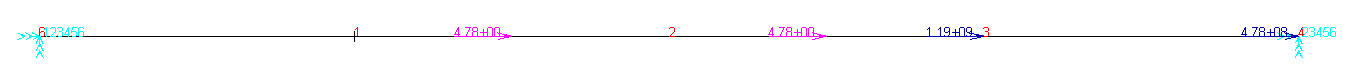
\includegraphics[width = \linewidth]{pic7.1.PNG}
            \caption{Модель стержня}
            \label{pic7.1}
        \end{center}
    \end{figure}

    \item Генерация фходного файла для расчета в MSC Nastran
    
    [Analysis] $\rightarrow$ [Action: Analyze] $\rightarrow$ [Object: Entire Model] $\rightarrow$ [Method: Full Run] $\rightarrow$ [Job Name: dz] $\rightarrow$ [Solution Type: Linear Static] $\rightarrow$ [Apply].

    \item Передача результатов расчета в MSC Patran
    
    [Action: Access Results] $\rightarrow$ [Object: Attach HDF5 XDB] $\rightarrow$ [Method: Result Entities] $\rightarrow$ [Job Name: dz] $\rightarrow$ [Select Results File: dz.h5 xdb] $\rightarrow$ [OK] $\rightarrow$ [Apply].
\end{enumerate}

Получим графики перемещений и нормальных напряжений:
\begin{figure}[H]
    \begin{center}
        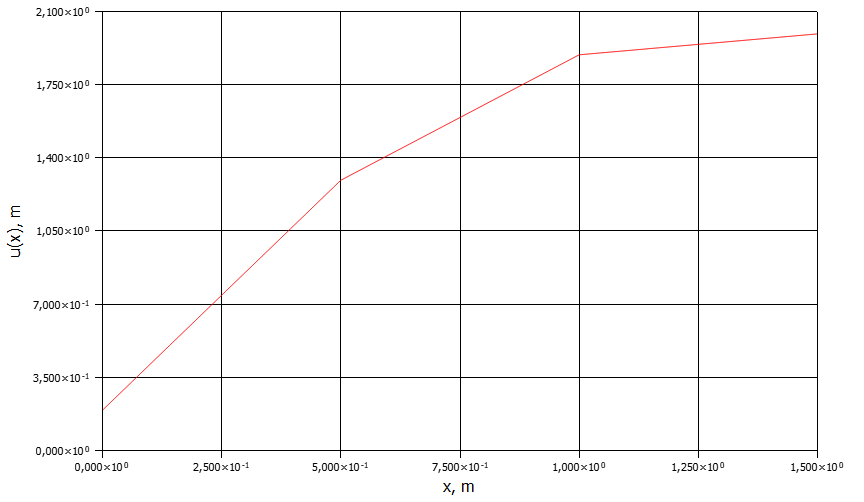
\includegraphics[width = 0.7\linewidth]{pic7.2.PNG}
        \caption{График перемещений}
        \label{pic7.2}
    \end{center}
\end{figure}
\begin{figure}[H]
    \begin{center}
        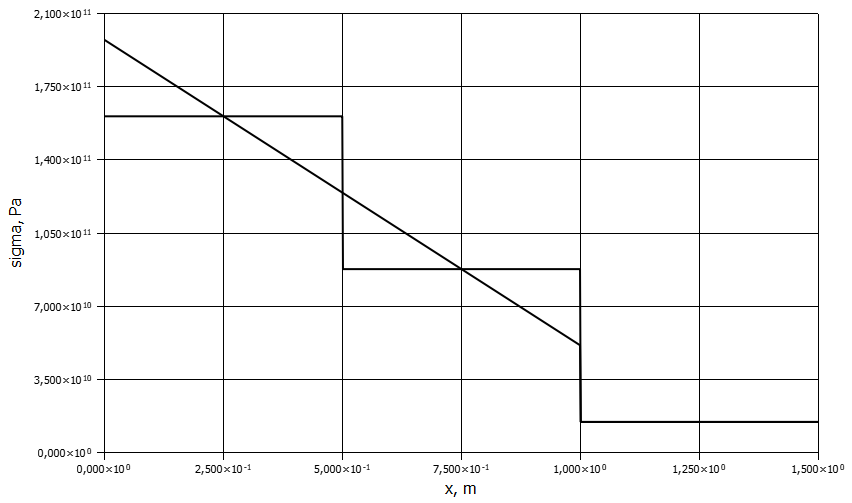
\includegraphics[width = 0.7\linewidth]{pic7.3.PNG}
        \caption{График нормальных напряжений}
        \label{pic7.3}
    \end{center}
\end{figure}

\section{Сравнительный анализ результатов, полученных методами, использованными в работе}

\begin{figure}[H]
    \begin{center}
        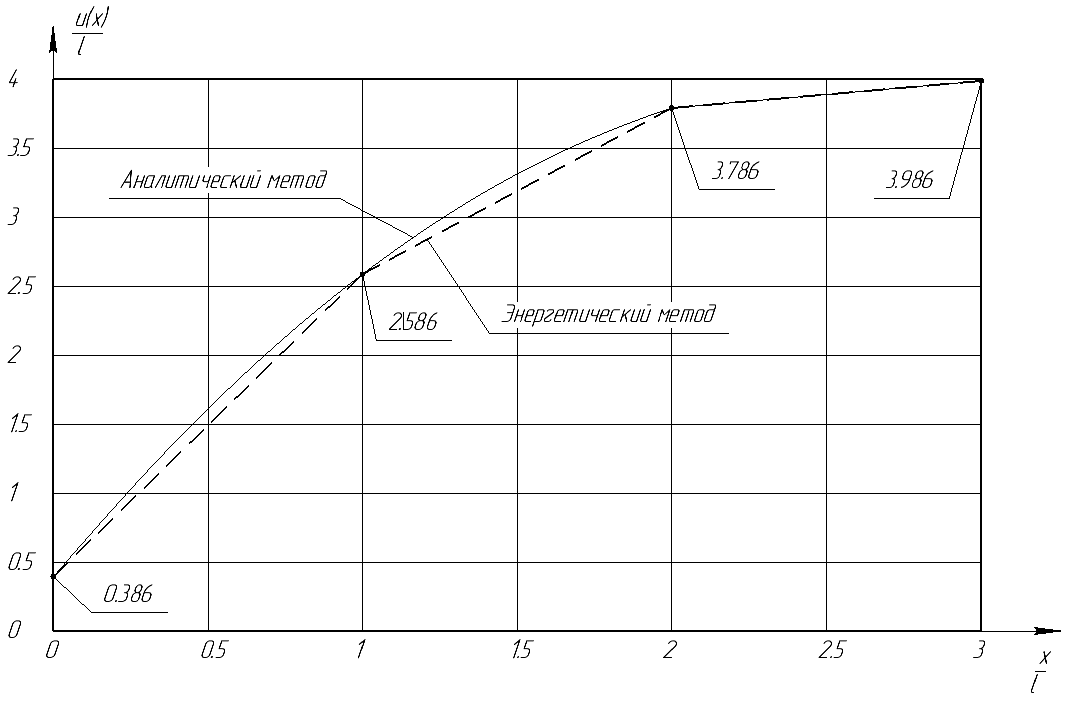
\includegraphics[width = 0.7\linewidth]{pic4.1.PNG}
        \caption{Сравнительный график аналитического и энергетического методов нахождения перемещений}
        \label{pic7.3.1}
    \end{center}
\end{figure}
\begin{figure}[H]
    \begin{center}
        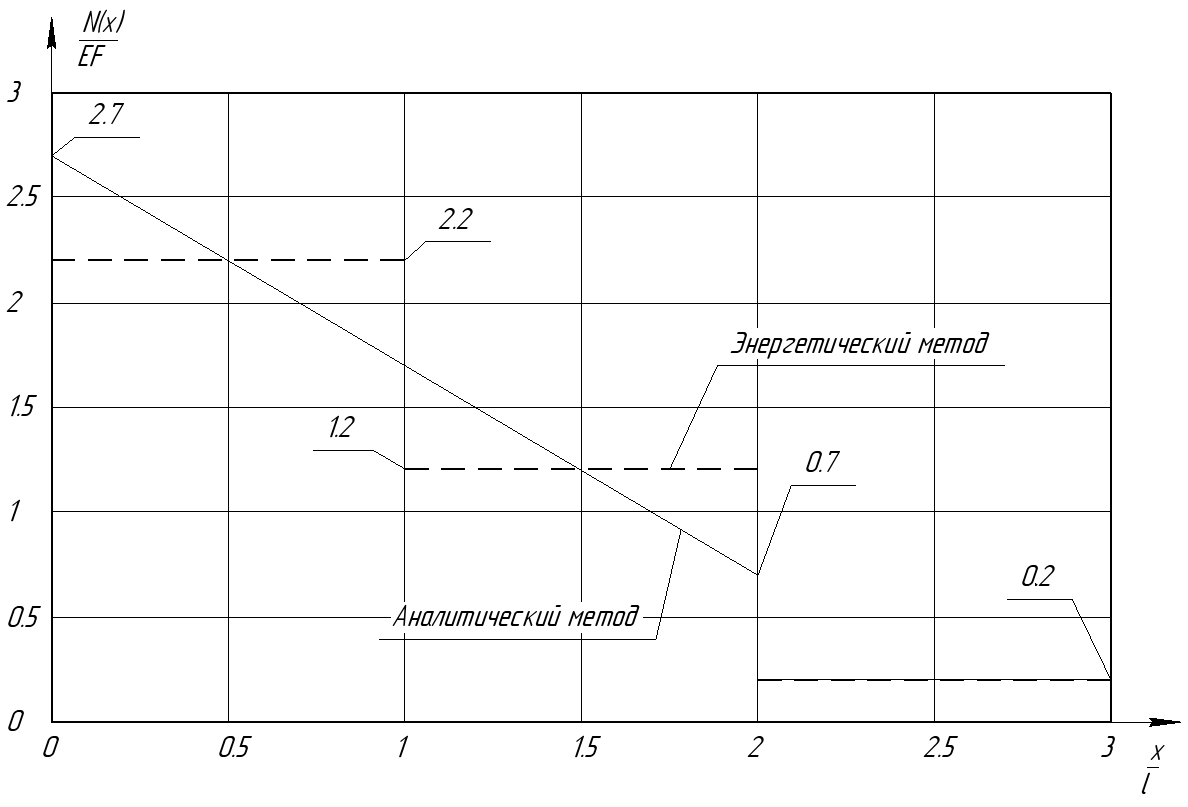
\includegraphics[width = 0.7\linewidth]{pic4.2.PNG}
        \caption{Сравнительный график аналитического и энергетического методов нахождения нормальных напряжений}
        \label{pic7.3.2}
    \end{center}
\end{figure}

Аналитическое решение дает результат на всем промежутке стрержня, в то время как энергетический метод и МКЭ дают результат только в конкретных точках, на которые разбивается модель. Для сравнения методов приведем таблицу со значениями перемещений и нормальных сил, полученными каждым методом:
\begin{table}[H]
    \caption{Сравнительная таблица перемещений}
    \label{tab7.1}
    \begin{center}
        \begin{tabular}{|c|c|c|c|}
            \hline
            Координата точки $x$, м & Аналитический метод & Энергетический метод & Patran \\
            \hline
            $0$ & $0.193$ & $0.192857$ & $0.1928439$ \\
            \hline
            $0.5$ & $1.293$ & $1.292857$ & $1.292854$ \\
            \hline
            $1$ & $1.893$ & $1.892857$ & $1.892836$ \\
            \hline
            $1.5$ & $1.993$ & $1.992857$ & $1.992841$ \\
            \hline
        \end{tabular}
    \end{center}
\end{table}
\begin{table}[H]
    \caption{Сравнительная таблица нормальных напряжений}
    \label{tab7.2}
    \begin{center}
        \begin{tabular}{|c|c|c|c|}
            \hline
            Координата точки, м & Аналитический метод & Энергетический метод и МКЭ & Patran \\
            \hline
            $0$ & $1.9737 \cdot 10^{11}$ & $1.6082 \cdot 10^{11}$ & $1.973735 \cdot 10^{11}$ \\
            \hline
            $0.5 - 0$ & $1.2427 \cdot 10^{11}$ & $1.6082 \cdot 10^{11}$ & $1.242694 \cdot 10^{11}$ \\
            \hline
            $0.5 + 0$ & $1.2427 \cdot 10^{11}$ & $8.772 \cdot 10^{10}$ & $1.242694 \cdot 10^{11}$ \\
            \hline
            $1 - 0$ & $5.117 \cdot 10^{10}$ & $8.772 \cdot 10^{10}$ & $5.116525 \cdot 10^{10}$ \\
            \hline
            $1 + 0$ & $1.462 \cdot 10^{10}$ & $1.462 \cdot 10^{10}$ & $1.462083 \cdot 10^{10}$ \\
            \hline
            $1.5$ & $1.462 \cdot 10^{10}$ & $1.462 \cdot 10^{10}$ & $1.462083 \cdot 10^{10}$ \\
            \hline
        \end{tabular}
    \end{center}
\end{table}